\documentclass[main.tex]{subfiles}

\begin{document}
\sloppy


\vspace{1.0cm}

\section{Redesign gerarchia dei FixtureComponent}\label{sec:FixtureComponentHierachy}
I FixtureComponent formano uno strato che si pone tra i dati DMX che arrivano ad UnrealEngine ed i materiali visti nel capitolo precedente. Mentre i materiali Light/Lens/Beam definiscono come effettuare il rendering della luce emessa da un faro, i FixtureComponent ne controllano i comportamenti e comunicano con i primi attraverso i parametri presenti nei vari moduli della pipeline che abbiamo creato in precedenza. Un altro modo che i FixtureComponent hanno per interagire con un faro istanziato in un mondo virtuale è andando direttamente a modificarne le proprietà (Ad esempio la rotazione delle varie geometrie). \newline

In questo capitolo analizzeremo i problemi riscontrati nell'implementazione di un nuovo componente e proporremo una nuova gerarchia atta all'aggiunta di nuove features nella maniera più semplice possibile.

\subsection{Vecchia implementazione}\label{subsec:3_oldImplementation}
I FixtureComponent sono, realmente, delle classi organizzate in una struttura gerarchica. Alla base abbiamo \lstinline{FixtureComponentBase}, esteso da \lstinline{SimpleAttributeFixtureComponent} (Ovvero singole features che vengono controllate in maniera diretta) e da \lstinline{MultipleAttributeFixtureComponent} (Ovvero features che vengono controllate da più canali, oppure che possono avere comportamenti avanzati).
\begin{figure}[H]
    \centering
    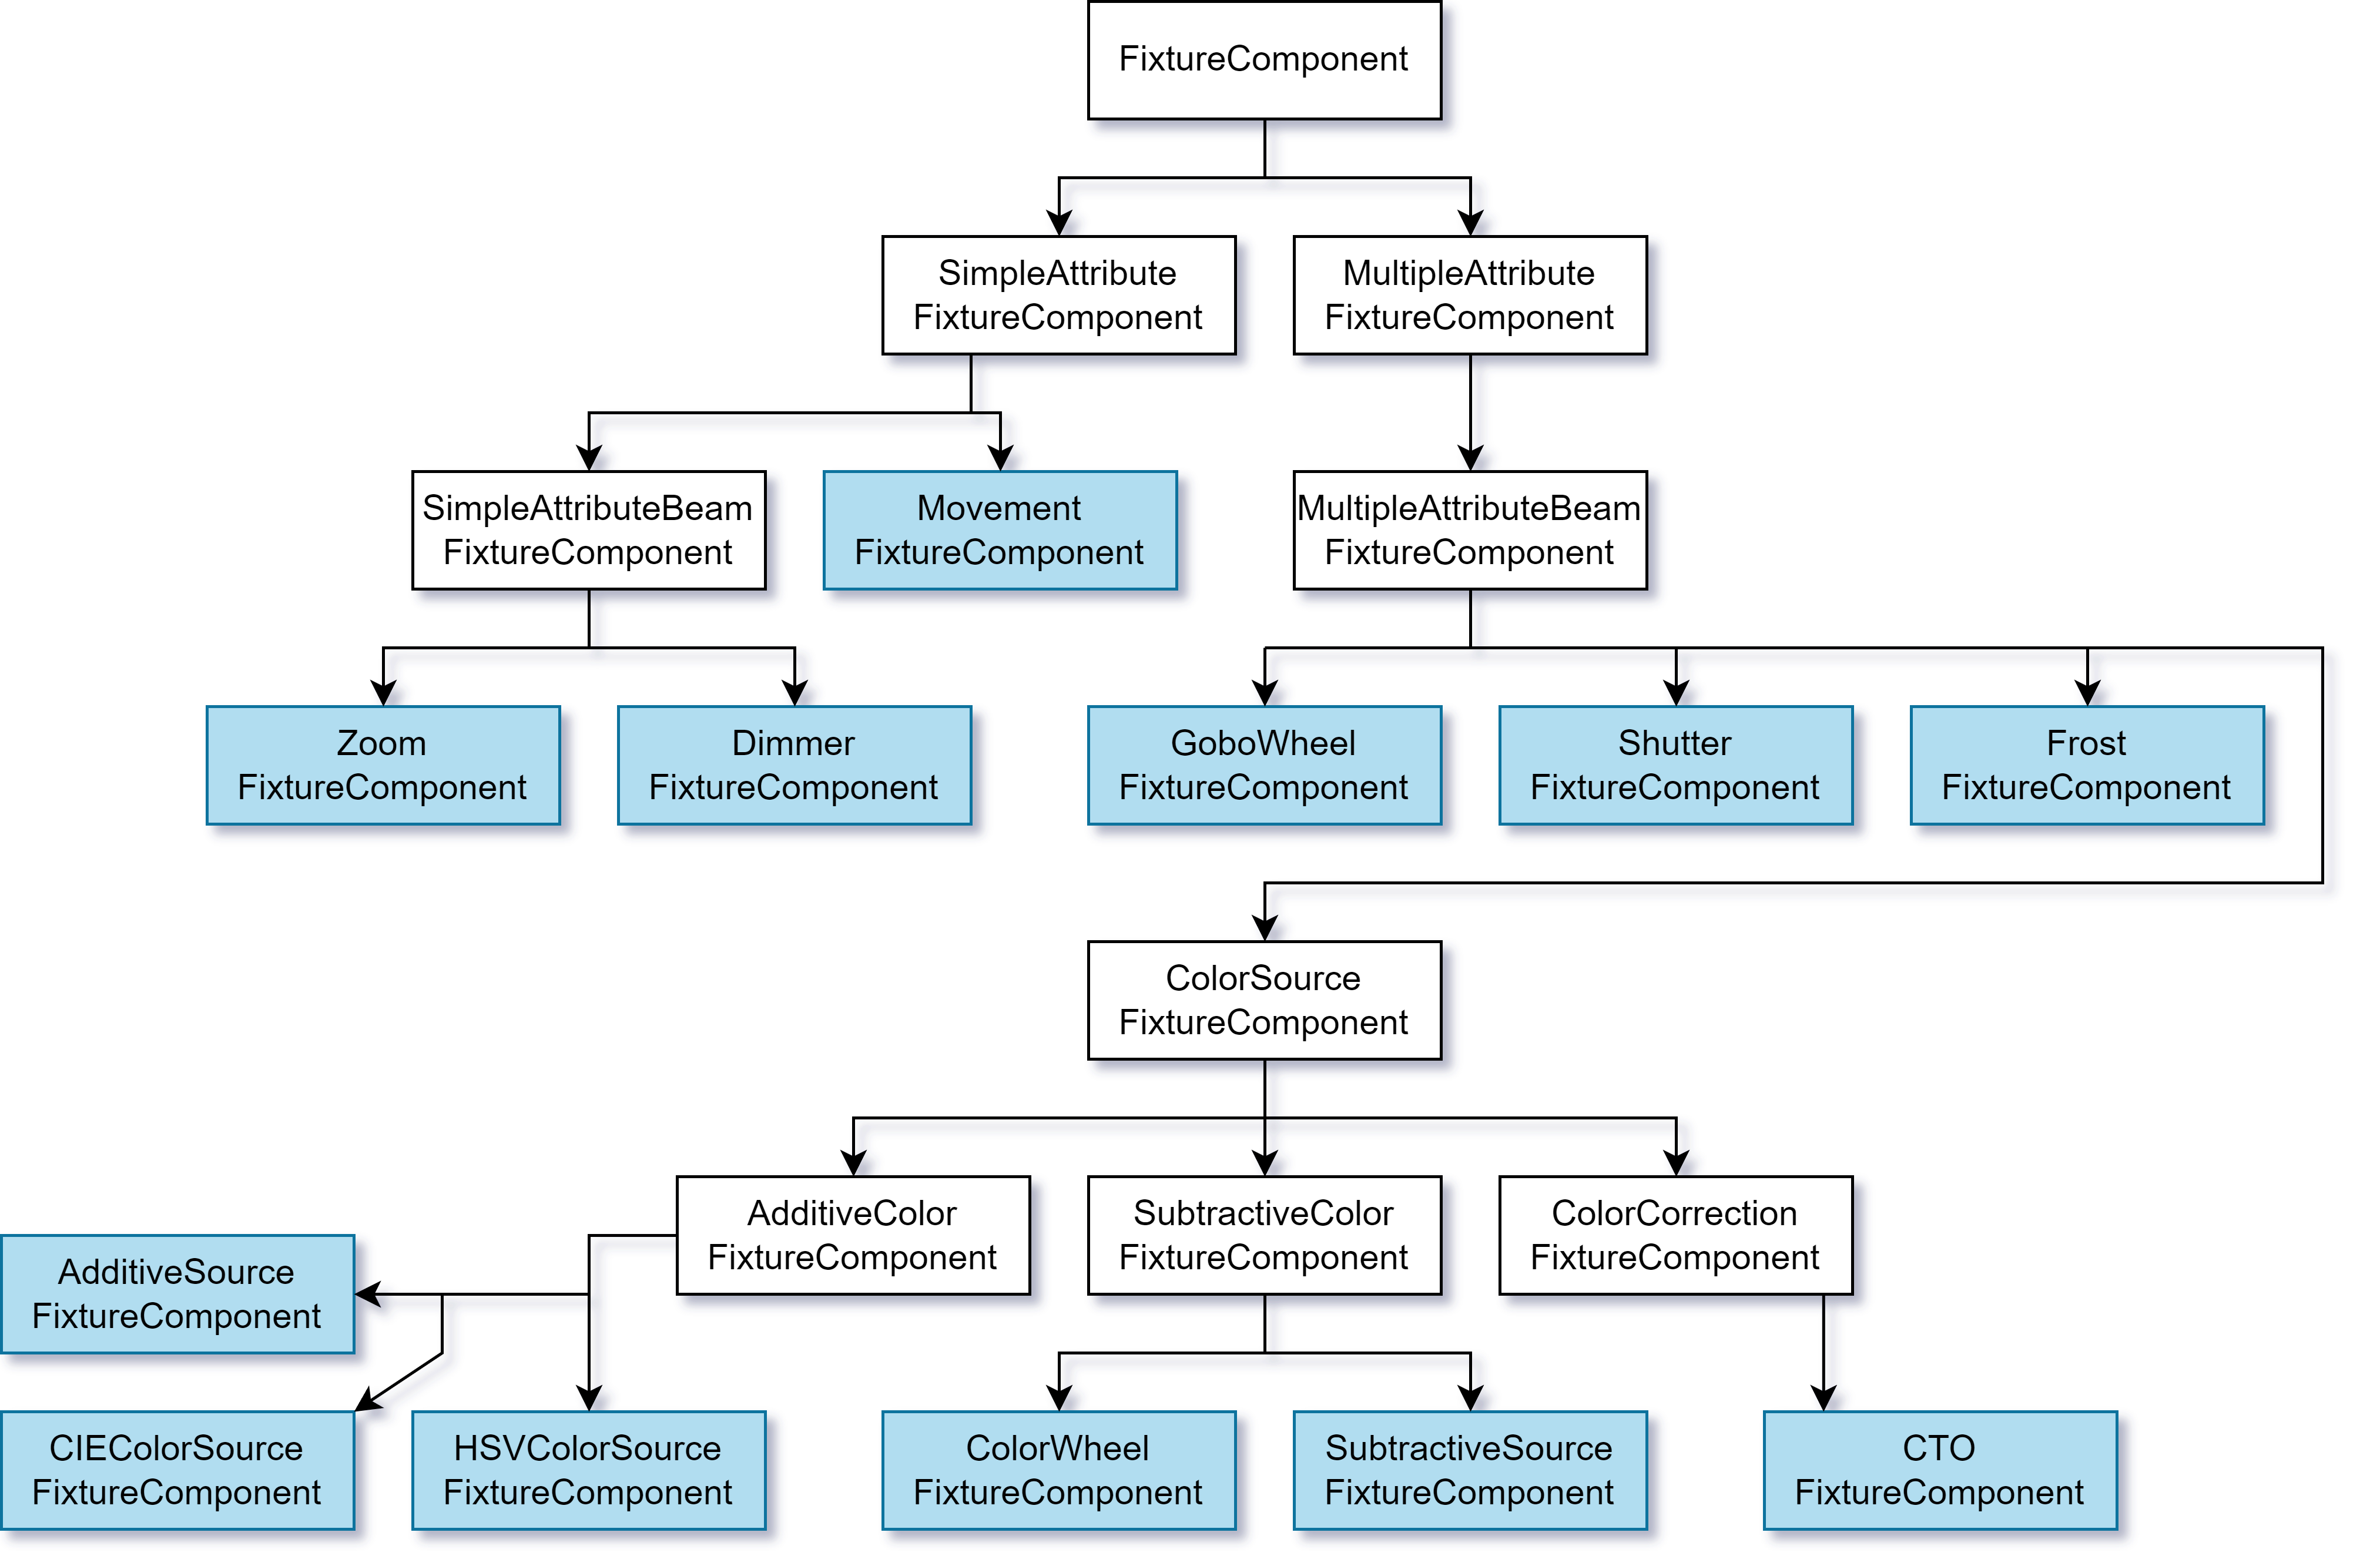
\includegraphics[width=0.9\linewidth]{img/fixtureComponent/FixtureComponentOLD.drawio.png}
    \caption{Struttura gerarchica delle classi FixtureComponent. In azzurro i componenti veri e propri.}
    \label{fig:3_fixtureComponentOld}
\end{figure}

%TODO descrivere in maniera "rapida" come funziona a runtime la gerarchia, attualmente

Analizzando l'implementazione di questa gerarchia sono sorte delle criticità:
\begin{itemize}
    \item \textbf{Codice duplicato}: Nonostante alcune funzioni siano state dichiarate (come virtuali) in una classe padre, molte classi figlie le reimplementano in maniera identica l'una dall'altra. Un esempio è la funzione \lstinline{} che viene definita nello stesso identico modo da tutti i figli diretti di \lstinline{MultipleAttributeFixtureComponent}:
\lstset{language=UEcpp}
\begin{lstlisting}
void UCPGDTFFrostFixtureComponent::PushDMXRawValues(
        UDMXEntityFixturePatch* FixturePatch,
        const TMap<int32, int32>& RawValuesMap) {

	int32* DMXValuePtr = RawValuesMap.Find(this->ChannelAddress);
	if (DMXValuePtr) this->ApplyEffectToBeam(*DMXValuePtr);
}

void UCPGDTFShutterFixtureComponent::PushDMXRawValues(
        UDMXEntityFixturePatch* FixturePatch,
        const TMap<int32, int32>& RawValuesMap) {

	int32* DMXValuePtr = RawValuesMap.Find(this->ChannelAddress);
	if (DMXValuePtr) this->ApplyEffectToBeam(*DMXValuePtr);
}
\end{lstlisting}
    \item \textbf{Virtualizzazione delle funzioni quasi assente}: Molte funzioni sono presenti su vari componenti della gerarchia, ma non sono mai dichiarate su una classe padre, nonostante facciano la stessa cosa ed è giusto che siano esposte agli altri componenti. Un esempio sono \lstinline{ApplyEffectToBeam} e \lstinline{SetTargetValue} che sono implementate da molti componenti, ma mai definiti in un padre (E sono anche un altro esempio di codice completamente duplicato) 
    \item \textbf{Elementi superflui nella gerarchia}: Elementi come Simple o Multiple AttributeBeamFixtureComponent sono essenzialmente vuoti e non portano miglioramenti alla definizione implicita della gerarchia %TODO CHIEDERE A DAVIDE COME SCRIVERE
    \item \textbf{Nessuna centralizzazione della gestione delle features}: La gerarchia viene definita attraverso delle classi che di fatto sono quasi delle interfacce. Questo comporta che la gestione di tutto che ci sta attorno ad una feature è a carico dei singoli componenti finali. Ogni volta che si implementa un nuovo componente si è quindi obbligati a rimplementare tutta la logica che sta dietro la gestione degli stessi.
    \item \textbf{Bassa chiarezza su cosa deve essere implementato nella singola feature}: Visti i punti precedenti, se si vuole implementare un nuovo componente (senza avere conoscenze pregresse) si rimane interdetti poiché non si capisce esattamente cosa bisogna fare per la realizzazione dello stesso. Non è presente una lista ben definita di funzionalità in cui il singolo componente deve specializzarsi.
    \item \textbf{Errori veri e propri nel calcolo di valori utili}: In generale, sono state riscontrate grosse mancanze con il calcolo di valori utili ad un componente. Ad esempio, il valore di minimo e massimo di una ChannelFunction viene calcolato solamente su quella corrente, piuttosto di avere un valore globale per tutti gli attributi dello stesso tipo. Oppure, i valori di fade e accelerazione per l'interpolazione non venivano proprio calcolati né presi dal GDTF originale.
    \item \textbf{Interpolazione mancante su molti componenti}: L'interpolazione non è gestita nella maniera corretta, di conseguenza è completamente mancante su molte feature di un faro (Ad esempio zoom, o rotazione di una gobo). Più specificatamente, è presente solamente sui componenti che estendono \lstinline{MultipleAttributesFixtureComponent} e se uno stesso componente controlla più features è attiva solo su una delle due
\end{itemize}

Per risolvere queste criticità è stato deciso un redesign dei vari FixtureComponent. A livello gerarchico non ci saranno molte differenze; esse saranno presenti maggiormente lato implementazione.

\subsection{Idea di reimplementazione}\label{subsec:3_idea}
Idealmente un componente dovrebbe definire pochi comportamenti specializzanti:
% TODO lista
Tutto il resto invece dovrebbe essere appannaggio dei padri, principalmente di \lstinline{FixtureComponentBase}
%TODO spiegazione precisa di fcbase

\subsubsection{Strutture dati}\label{subsec:3_2_structs}

\subsection{Implementazione}\label{subsec:3_implementation}
\subsubsection{Ottenimento valori di default per le varie funzionalità di una fixture}\label{subsec:3_1_defaultValues}

\end{document}